\documentclass[14pt,a4paper,report]{report}
\usepackage[a4paper, mag=1000, left=2.5cm, right=1cm, top=2cm, bottom=2cm, headsep=0.7cm, footskip=1cm]{geometry}
\usepackage[utf8]{inputenc}
\usepackage[english,russian]{babel}
\usepackage{indentfirst}
\usepackage[dvipsnames]{xcolor}
\usepackage[colorlinks]{hyperref}
\usepackage{listings} 
\usepackage{fancyhdr}
\usepackage{caption}
\usepackage{amsmath}
\usepackage{graphicx}
\usepackage{amsmath}
\usepackage{booktabs}
\usepackage{array}
\newcolumntype{P}[1]{>{\centering\arraybackslash}p{#1}}
\hypersetup{
	colorlinks = true,
	linkcolor  = black
}

\usepackage{titlesec}
\titleformat{\chapter}
{\Large\bfseries} % format
{}                % label
{0pt}             % sep
{\huge}           % before-code


\DeclareCaptionFont{white}{\color{white}} 

% Listing description
\usepackage{listings} 
\DeclareCaptionFormat{listing}{\colorbox{gray}{\parbox{\textwidth}{#1#2#3}}}
\captionsetup[lstlisting]{format=listing,labelfont=white,textfont=white}
\lstset{ 
	% Listing settings
	inputencoding = utf8,			
	extendedchars = \true, 
	keepspaces = true, 			  	 % Поддержка кириллицы и пробелов в комментариях
	language = C,            	 	 % Язык программирования (для подсветки)
	basicstyle = \small\sffamily, 	 % Размер и начертание шрифта для подсветки кода
	numbers = left,               	 % Где поставить нумерацию строк (слева\справа)
	numberstyle = \tiny,          	 % Размер шрифта для номеров строк
	stepnumber = 1,               	 % Размер шага между двумя номерами строк
	numbersep = 5pt,              	 % Как далеко отстоят номера строк от подсвечиваемого кода
	backgroundcolor = \color{white}, % Цвет фона подсветки - используем \usepackage{color}
	showspaces = false,           	 % Показывать или нет пробелы специальными отступами
	showstringspaces = false,    	 % Показывать или нет пробелы в строках
	showtabs = false,           	 % Показывать или нет табуляцию в строках
	frame = single,              	 % Рисовать рамку вокруг кода
	tabsize = 2,                  	 % Размер табуляции по умолчанию равен 2 пробелам
	captionpos = t,             	 % Позиция заголовка вверху [t] или внизу [b] 
	breaklines = true,           	 % Автоматически переносить строки (да\нет)
	breakatwhitespace = false,   	 % Переносить строки только если есть пробел
	escapeinside = {\%*}{*)}      	 % Если нужно добавить комментарии в коде
}

\begin{document}

\def\contentsname{Содержание}

% Titlepage
\begin{titlepage}
	\begin{center}
		\textsc{Санкт-Петербургский Политехнический 
			Университет Петра Великого\\[5mm]
			Кафедра компьютерных систем и программных технологий}
		
		\vfill
		
		\textbf{Отчёт по лабораторной работе №3.2\\[3mm]
			Курс: «Разработка экспертной системы с нуля»\\[41mm]
		}
	\end{center}
	
	\hfill
	\begin{minipage}{.4\textwidth}
		Выполнил студент:\\[2mm] 
		Бояркин Н.С.\\
		Группа: 13541/3\\[5mm]
		
		Проверил:\\[2mm] 
		Сазанов А.М.
	\end{minipage}
	\vfill
	\begin{center}
		Санкт-Петербург\\ \the\year\ г.
	\end{center}
\end{titlepage}

% Contents
\tableofcontents
\clearpage

\chapter{Лабораторная работа №3.2}

\section{Цель работы}

Научиться создавать экспертные системы с помощью конструктора Exsys CORVID.

\section{Программа работы}

\begin{enumerate}
	\item Разработайте экспертную систему для своего варианта индивидуального задания.
	\item Можно ли решить поставленную задачу проще без использования ЭС?
	\item В каких областях, по Вашему мнению, использование ЭС потенциально опасно (или вредно)?
\end{enumerate}

\clearpage

\section{Ход работы}

\subsection{Разработайте экспертную систему для своего варианта индивидуального задания}

\textbf{Тема 1.} Экспертная система по определению оптимальной конфигурации ПК. Возможные входные данные для ЭС:

\begin{enumerate}
	\item Цели использования ПК.
	\item Максимальный бюджет на выбранную конфигурацию.
	\item Изготовитель комплектующих.
\end{enumerate}

Разработаем логическую схему работы требуемой экспертной системы. Система состоит из основного логического блока и 10 логических блоков для формирования конкретных списков покупок. Рассмотрим основной логический блок:

\begin{figure}[h!]
	\centering
	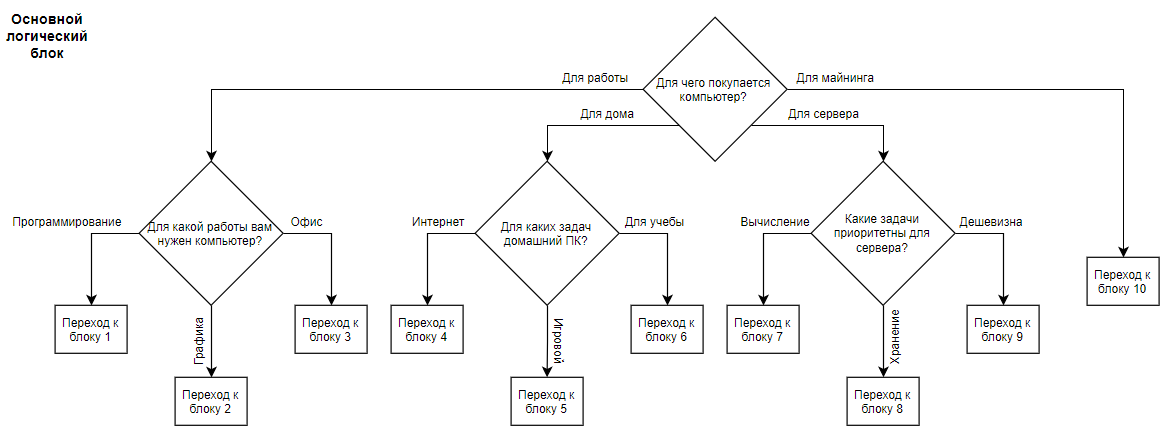
\includegraphics[scale = 0.55]{images/0_1.png}
	\caption{Структура основного логического блока}
\end{figure}

Рассмотрим работу остальных логических блоков:

\begin{figure}[h!]
	\centering
	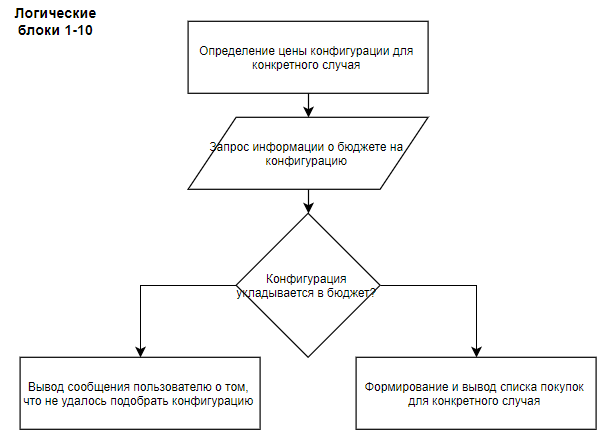
\includegraphics[scale = 0.65]{images/0_2.png}
	\caption{Структура логических блоков для конкретных сценариев}
\end{figure}

Таким образом в экспертной системе реализовано 20 различных сценариев.

Таким образом, пользователь определяет цели использования компьютера, после чего вводит информацию о бюджете. Если конфигурация для конкретной цели укладывается в бюджет, то формируется список покупок и выводится пользователю. Если нет, то пользователь уведомляется о том, что бюджет слишком мал.

Реализация основного логического блока:

\begin{figure}[h!]
	\centering
	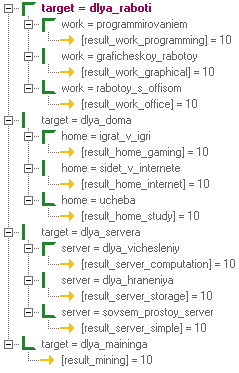
\includegraphics[scale = 0.90]{images/1.png}
	\caption{Реализация основного логического блока}
\end{figure}

Пример реализации одного из 10 логических блоков для конкретного сценария:

\begin{figure}[h!]
	\centering
	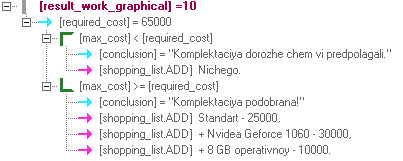
\includegraphics[scale = 0.95]{images/2.png}
	\caption{Пример реализации логического блока для конкретного сценария}
\end{figure}

В данном случае, пользователь определяется с целью и выбирает компьютер для графической работы. После чего вычисляется необходимая цена 65000. Далее пользователь вводит максимальный бюджет и производится сравнение с необходимой ценой. Если цена укладывается в бюджет, то формируется список покупок, а если нет, то выводится сообщение о неудаче.

Текст, выводимый на экран практически полностью определяется введенными переменными:

\begin{figure}[h!]
	\centering
	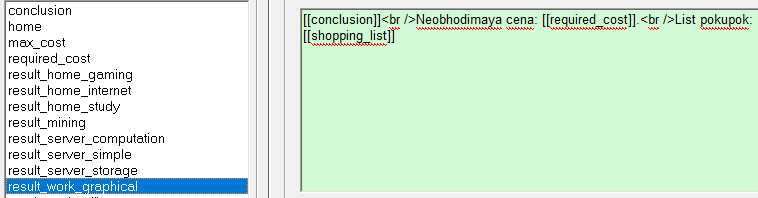
\includegraphics[scale = 0.85]{images/3.png}
	\caption{Шаблон для вывода на экран}
\end{figure}

Рассмотрим работу системы на примере этого сценария:

\begin{figure*}[ht!]
	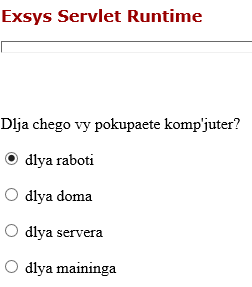
\includegraphics[width=.30\textwidth]{images/4.png}\hfill
	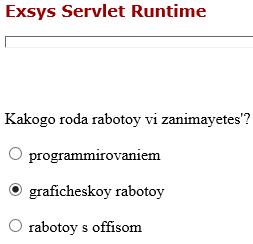
\includegraphics[width=.35\textwidth]{images/5.png}
	\caption{Определение задачи компьютера}
\end{figure*}

\begin{figure}[h!]
	\centering
	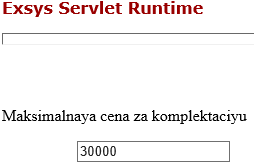
\includegraphics[scale = 0.90]{images/6.png}
	\caption{Ввод информации о бюджете}
\end{figure}

\begin{figure}[h!]
	\centering
	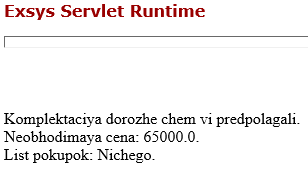
\includegraphics[scale = 0.90]{images/7.png}
	\caption{Если комплектация не укладывается в бюджет}
\end{figure}

\begin{figure}[h!]
	\centering
	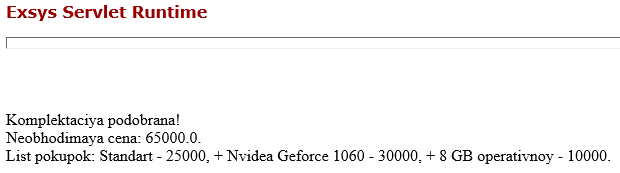
\includegraphics[scale = 0.90]{images/8.png}
	\caption{Если комплектация укладывается в бюджет}
\end{figure}

\subsection{Можно ли решить поставленную задачу проще без использования ЭС?}

Существующие варианты в этой области:

\begin{enumerate}
	\item Хороший вариант -- Программы, которые анализируют популярные (на данный момент) стабильные комплектации и классифицируют их по различным параметрам и для различных целей. После чего пользователь уже выбирает из очень ограниченного числа вариантов.
	\item Идеальный вариант -- Консультант человек. 
\end{enumerate}

Первый вариант все таки требует некоторых знаний от пользователя в области подбора комплектующих, однако, для чуть более опытных пользователей этот вариант подходит лучше всего.

Второй вариант для неопытного пользователя является наилучшим. На практике найти консультанта не так уж и сложно -- в технических магазинах, на форуме, в онлайн магазинах, среди знакомых и т.д.

\subsection{В каких областях, по Вашему мнению, использование ЭС потенциально опасно (или вредно)?}

\begin{itemize}
	\item В областях, где накопленные знания быстро меняются или устаревают.
	\item В областях, где необходимо принятие незамедлительного решения, основанного на опыте и умении специалиста.
	\item В очень широких областях, где продолжительность диалога с пользователем стремится к бесконечности.
\end{itemize}

\section{Вывод}

В результате работы была успешно реализована ЭС для задачи подбора комплектующих к компьютеру. В ходе работы использовались различные виды переменных: статические списки, коллекции, числовые и текстовые переменные. Кроме того, было задействовано множество логических блоков, для разгрузки основной логики. Данное решение повысило модульность и наблюдаемость системы.

Использование ЭС для реализации задачи подбора комплектующих не очень верное решение, так как рынок быстро меняется и появляются новые технологии. Кроме того, количество различных нюансов и альтернатив при выборе комплектующих делает диалог с пользователем долгим и неэффективным.

\section{Список литературы}

% \linebreak

\begin{flushleft}
	
[1] РАЗРАБОТКА ЭКСПЕРТНЫХ СИСТЕМ, О.А. ТАДЖИБАЕВА [Электронный ресурс]. — URL: \href{http://artlib.osu.ru/web/metod/655_20110711.pdf}{http://artlib.osu.ru/web/metod/655\_20110711.pdf} (дата обращения 21.10.2017). \linebreak

\end{flushleft}
	


\end{document}